\begin{center} 
\emph{``To be trusted is a greater compliment than being loved.'' -- George MacDonald}
\end{center}

\section{Orthogonality}\label{sec:ortho}
\centerline{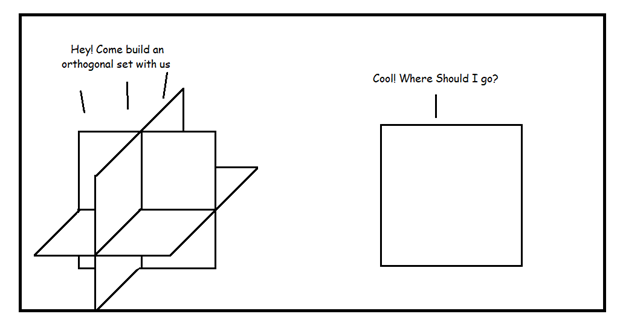
\includegraphics[scale=0.75]{Chapter4/images/orthocomic.png}}
%{\vspace{-10 pt}\hfill\footnotesize (Image contributed by Thayne Hansen)}\\
\begin{Def} Two nonzero\footnotemark[2] vectors $\bb u, \bb v\in F^n$ are \textbf{orthogonal} if $\bb u\cdot \bb v=0$.
\end{Def}\vs

\begin{Exam} Given the vectors $\bb u = \vr{1\\2\\3}$, $\bb v= \vr{1\\1\\-1}$, and $\bb w = \vr{2\\3\\5}$, determine if $\bb u$ is orthogonal to $\bb v$ or $\bb w$.\\
\[\bb u \cdot \bb v = 1(1)+2(1)+3(-1) = 3-3 = 0.\] Thus, $\bb u$ is orthogonal to $\bb v$. 
\[\bb u \cdot \bb w = 1(2)+2(3)+3(5) = 23\neq 0.\] Thus, $\bb u$ is not orthogonal to $\bb w$.
\[\bb v \cdot \bb w = 1(2)+1(3)-1(5) = 5-5 = 0.\] Thus, $\bb v$ is orthogonal to $\bb w$. 
\end{Exam}\vs

\begin{Thm}[Pythagorean Theorem] \label{thm:pythagorean}
Two vectors $\bb u, \bb v\in F^n$ are orthogonal\footnotemark[8] then \[\Vert \bb u + \bb v\Vert^2 = \Vert \bb u\Vert^2+ \Vert \bb v\Vert^2.\]
\end{Thm}
%\begin{Thm}[Pythagorean Theorem] 
%Two vectors $\bb u, \bb v\in V$ are orthogonal if and only if \[\Vert \bb u + \bb v\Vert^2 = \Vert \bb u\Vert^2+ \Vert \bb v\Vert^2.\]
%\end{Thm}
\begin{proof}By assumption, $\bb u\cdot \bb v =0 = \overline{\bb u\cdot\bb v} = \bb v\cdot \bb u$. Note that
$\Vert \bb u + \bb v\Vert^2 = (\bb u + \bb v)\cdot(\bb u + \bb v) = \bb u\cdot \bb u + \bb u\cdot \bb v + \bb v\cdot \bb u + \bb v\cdot \bb v = \bb u\cdot \bb u + 0 + 0+ \bb v\cdot \bb v = \Vert \bb u\Vert^2+ \Vert \bb v\Vert^2.$  
\end{proof}\vs

We call the above equation the Pythagorean Theorem because how it resembles the trigonometric equation, after all it states that a sum of squares is equal to a square under certain conditions, but there is a deeper geometry connection. First of all, if two vectors $\bb u$ and $\bb v$ are linearly independent, then they span a plane in $\R^n$, but they also form a triangle with sides $\bb u$, $\bb v$, and $\bb u + \bb v$, where the three points correspond to the tail of $\bb u$ (which is also the tail of $\bb u + \bb v$), the head of $\bb u$ (which is also the tail of $\bb v$), and the head of $\bb v$ (which is also the head of $\bb u + \bb v$). The lengths of the three sides of this triangle is $\Vert \bb u\Vert$, $\Vert \bb v\Vert$, and $\Vert \bb u + \bb v\Vert$. Therefore, the above theorem is saying that the sums of squares of two sides of the a triangle equal the square of the other side. This is exactly the statement of the Pythagorean Theorem from Trigonometry, but furthermore the Trigonometric Pythagorean Theorem guarantees this can only happen if there is a right angle present, that is, the angle between the vectors $\bb u$ and $\bb v$ must be a right angle. This proves the notion that two vectors are orthogonal if and only if the angle between the two vectors is $90^\circ$.\\

An alternative way of expressing a plane in $F^3$ is by orthogonality. For example, we can construct a plane in $F^3$ by taking all vectors in $F^3$ that are orthogonal to some fixed vector $\bb n =(a,\ b,\ c)$, called the \textbf{normal vector} of the plane. If $\bb x = (x,\ y,\ z)$ is a vector on the plane, then 
\[\bb n \cdot \bb x = ax+by+cz = 0.\] This produces the equation of a plane which passes through the origin (notice that $\bb 0$ is a solution here). In order to have the plane pass through the particular vector $\bb x_0$ we replace $\bb x$ with $\bb x - \bb{x_0}$, that is, 
\begin{eqnarray*}
\bb n \cdot (\bb x - \bb{x_0}) &=& 0 \\
a(x-x_0) + b(y-y_0) + c(z-z_0) &=& 0\\
ax + by + cz &=& d, 
\end{eqnarray*} gives an equation of the plane in $F^3$ through the point $(x_0, y_0, z_0)$ and orthogonal to $\bb n$.\\

\begin{Exam} The solutions to the equation 
\[3(x-4) + 5(y+5) - 2z = 0 \qRightarrow 3x+5y-2z = -13\] is the plane containing the point $(4,-5,0)$ and is perpendicular to $(3, 5, -2)$.
\end{Exam}\vs

Similarly, this strategy will create a hyperplane in $F^n$. In particular, the hyperplane containing $\bb x_0$ and is orthogonal to $\bb n$ will be the solutions $\bb x$ to the linear equation, given in \textbf{point-normal form}, \begin{equation} \bb n\cdot (\bb x-\bb x_0)=0.\end{equation}\vs


\begin{Def} A set of nonzero vectors $\{\bb v_1, \ldots, \bb v_r\}\subseteq F^n$ is called an \textbf{orthogonal set} if each pair of distinct vectors is orthogonal, that is, $\bb v_i \cdot \bb v_j = 0$ whenever $i\neq j$. An orthogonal set of vectors is called \textbf{orthonormal} if each vector in the set is also a unit vector.
\end{Def}\vs


Of course, any orthogonal set can be transformed into an orthonormal set by normalizing each vector, that is, replacing each vector $\bb v$ with $\dfrac{1}{\Vert \bb v \Vert}\bb v$.\\

\begin{Exam}\label{exam:4.2orthobasis} Let  $\bb v_1 = \vr{1\\2\\3}, \bb v_2 = \vr{1\\1\\-1}, \bb v_3 = \vr{-5\\4\\-1}$. Then the set $\{\bb v_1, \bb v_2, \bb v_3\}$ is orthogonal with respect to the dot product. To see this, we check the three dot products:
\begin{eqnarray*}
\bb v_1\cdot \bb v_2 &=& 1+2-3 = 0\\
\bb v_1\cdot \bb v_3 &=& -5+8-3 =0\\
\bb v_2\cdot \bb v_3 &=& -5+4+1 = 0.
\end{eqnarray*}
\end{Exam}

%\begin{Thm} Let $V$ be an inner product space. If $S = \{\bb v_1, \ldots, \bb v_p\} \subseteq V$ is an orthogonal set of nonzero vectors, then $S$ is linearly independent.
%\end{Thm}
%\begin{proof}
%Suppose that 
%\[c_1\bb v_1 + c_2\bb v_2 + \ldots + c_p\bb v_p = \bb 0.\] Then for each $i$,
%\begin{eqnarray*}
%\langle c_1\bb v_1 + c_2\bb v_2 + \ldots + c_p\bb v_p,\  \bb v_i\rangle &=& \langle \bb 0,\  \bb v_i\rangle \\
%\langle c_1\bb v_1, \bb v_i\rangle  + \langle c_2\bb v_2, \bb v_i\rangle + \ldots + \langle c_i\bb v_i, \bb v_i\rangle + \ldots + \langle c_p\bb v_p, \bb v_i\rangle &=&  0\\
%c_1\langle \bb v_1, \bb v_i\rangle + c_2\langle \bb v_2, \bb v_i\rangle + \ldots + c_i\langle\bb v_i, \bb v_i\rangle + \ldots + c_p\langle \bb v_p, \bb v_i\rangle &=&  0\\
%0+ 0 + \ldots + c_i\Vert \bb v_i\Vert^2 + \ldots + 0 &=&  0\\
%c_i\Vert \bb v_i\Vert^2&=&  0. 
%\end{eqnarray*} Therefore, $c_i = 0$ or $\Vert \bb v_i\Vert = 0$. Since $\bb v_i\neq \bb 0$, the latter is impossible. Therefore, $c_i = 0$ for all $i$, which implies that $S$ is linearly independent.
%\end{proof}\vs

\begin{Thm}\label{thm:orthoindependent} If $S = \{\bb v_1, \ldots, \bb v_p\} \subseteq F^n$ is an orthogonal set of nonzero vectors, then $S$ is linearly independent.
\end{Thm}\vs
%\begin{proof}
%Suppose that 
%\[c_1\bb v_1 + c_2\bb v_2 + \ldots + c_p\bb v_p = \bb 0.\] Then for each $i$,
%\begin{eqnarray*}
%\bb v_i \cdot (c_1\bb v_1 + c_2\bb v_2 + \ldots + c_p\bb v_p) &=& \bb v_1\cdot  \bb 0 \\
%(\bb v_i \cdot c_i\bb v_1)  + ( \bb v_i\cdot c_2\bb v_2) + \ldots + ( \bb v_i\cdot c_i\bb v_i) + \ldots + ( \bb v_i\cdot c_p\bb v_p) &=&  0\\
%c_1( \bb v_i\cdot \bb v_1) + c_2( \bb v_i\cdot \bb v_2) + \ldots + c_i(\bb v_i\cdot \bb v_i) + \ldots + c_p( \bb v_i\cdot \bb v_p) &=&  0\\
%0+ 0 + \ldots + c_i\Vert \bb v_i\Vert^2 + \ldots + 0 &=&  0\\
%c_i\Vert \bb v_i\Vert^2&=&  0. 
%\end{eqnarray*} Therefore, $c_i = 0$ or $\Vert \bb v_i\Vert = 0$. Since $\bb v_i\neq \bb 0$, the latter is impossible. Therefore, $c_i = 0$ for all $i$, which implies that $S$ is linearly independent.
%\end{proof}\vs

The requirement that an orthogonal set contain only nonzero vectors is critical. Note that $\bb 0 \cdot \bb v=0$ for any vector $\bb v$. Thus, as we defined an orthogonal pair, the zero vector is orthogonal to every vector. This is a truly exceptional quality shared by no other vector. For this reason, the zero vector must be treated definitely in the theory of orthogonality and it is thus excluded from orthogonal sets. While this may seem somewhat arbitrary, this is truly consequence driven. The main consequence is that \thmref{thm:orthoindependent} would fail if $\bb 0$ were allowed in. It should also be noted that for a singleton $\{\bb v\}$, this set is orthogonal if and only if $\bb v\neq 0$, the same condition that guarantees that $\{\bb v\}$ is linearly independent. Notice that the condition that all pairs be orthogonal is vacuously true in this case as there are no pairs which are not orthogonal (since there are no pairs at all). This also holds for the empty set $\emptyset$. It has no pairs of distinct vectors which are not orthogonal, hence, the empty set is an orthogonal set.\\

An orthogonal (orthonormal) spanning set of $F^n$ is necessarily a basis, called an \textbf{orthogonal (orthonormal) basis}. For example, the standard basis in $F^n$ is an orthonormal basis.\\

\begin{Thm}\label{thm:orthocomplement} Let $W$ be a subspace of $F^n$. Let $W^\perp = \{\bb x\in F^n \mid \bb w\cdot \bb x  = 0,\; \forall\bb w\in W\}$, called the \textbf{orthogonal complement} of $W$. Then $W^\perp$ is also a subspace of $F^n$.
\end{Thm}\vs

\begin{Exam} Let $W$ be the $z$-axis in $\R^3$. Then $W^\perp$ is the $xy$-plane.
\end{Exam}\vs

\begin{Thm}\label{thm:rowortho} Let $A$ be an $m\times n$ matrix. Then 
\[(\row A)^\perp = \nul A.\footnotemark[3]\]
\end{Thm}\vs


\begin{Exam} Let $W$ be the subspace of $\R^6$ spanned by the vectors 
\[\bb w_1 = (1,3,-2,0,2,0),\ \bb w_2 = (2,6,-5,-2,4,-3),\ \bb w_3 = (0,0,5,10,0,15),\ \bb w_4 = (2,6,0,8,4,18).\] Construct a base for $W^\perp$.\\

We can arrange these vectors into a matrix $A$:
\[A = \mtx{rrrrrr}{1 & 3 & -2 & 0 & 2 & 0 \\ 2 & 6 & -5 & -2 & 4 & -3 \\ 0 & 0& 5 & 10 & 0 & 15 \\ 2 & 6 & 0 & 9 & 4 & 18} \sim \mtx{rrrrrr}{1 & 3 & 0 & 4 & 2 & 0\\ 0 & 0 & 1 & 2 & 0 &0 \\ 0 &0 & 0 &0 & 0 & 1\\ 0 &0 & 0 &0 & 0 & 0}\] such that $W = \row(A)$. By the previous result, $W^\perp = \row(A)^\perp = \nul(A)$. As we know how to find a basis for a null space given the echelon form of the matrix,  
\[W^\perp = \Span\{ (-3, 1, 0, 0, 0, 0),\ (-4, 0, -2, 1, 0, 0),\ (-2,0,0,0,1,0)\}. \qedhere\]
\end{Exam}\vs

Despite our reluctance to use any fields other than $\R$ and $\C$, the entirety of this section\footnotemark[9] is transferable to any field using the dot product or Hermitian product.

%%%%%%%%%%%%%%%%%% Exercises %%%%%%%%%%%%%%%%%%%
\startExercises{ortho}

\begin{enumerate}[!HW!, start=1]
\itemspade Find $k$ so that $\vr{k\\ 1}\cdot \vr{4\\3}$ is orthogonal in $\R^2$.
\end{enumerate}


\noindent For Exercises \ref{exer:hyperplaneorthostart}-\ref{exer:hyperplaneorthostop}, find a hyperplane in $F^n$ containing the vector $\bb x_0$, listed first, and whose normal vector is $\bb n$, listed second.
\begin{enumerate}[!HW!, label=$\spadesuit$ \arabic*., ref=\arabic*]
\begin{multicols}{3}
\item\label{exer:hyperplaneorthostart} $\vr{1\\2\\3}$, $\vr{3\\-2\\0}$ 
\itemspade $\vr{0\\0\\1\\2}$, $\vr{1\\-2\\2\\-1}$
\item\label{exer:hyperplaneorthostop} $\vr{1\\2\\3\\4\\5}$, $\vr{-3\\-6\\3\\2\\-5}$
\end{multicols}
\end{enumerate}
\begin{enumerate}[!HW!]
\item $\vr{10\\-8\\6\\-4\\2}$, $\vr{1\\3\\5\\7\\9}$ %Kennedy Worthington
\end{enumerate}

\noindent For Exercises \ref{exer:orthocomplstart}-\ref{exer:orthocomplstop}, find a basis for the orthogonal complement of $W$. Answers may vary.
\begin{enumerate}[!HW!, label=$\spadesuit$ \arabic*., ref=\arabic*] %Hefferon??
\begin{multicols}{2}
\item\label{exer:orthocomplstart}  $W = \Span\left\{\vr{0\\2\\0}, \vr{1\\-1\\1}\right\} \le \R^3$
\itemspade $W = \Span\left\{\vr{1\\3\\-1}\right\} \le \R^3$
\end{multicols}
\begin{multicols}{2}
\itemspade $W = \left\{\vr{x_1\\x_2}\ \middle|\  x_1+x_2=0\right\} \le \R^2$
\itemspade $W = \left\{\vr{x_1\\x_2}\ \middle|\ -2x_1+3x_2=0\right\} \le \R^2$
\end{multicols}
\begin{multicols}{2}
\itemspade $W = \left\{\vr{x_1\\x_2\\x_3}\ \middle|\ -x_1+3x_2+x_3=0\right\} \le \R^3$
\item\label{exer:orthocomplstop} $W = \left\{\vr{x_1\\x_2\\x_3}\ \middle|\ x_1=0, x_2+x_3=0\right\} \le \R^3$
\end{multicols}
\end{enumerate}

%%%%%%%%%%%%%%%%%%% Footnotes %%%%%%%%%%%%%%%%%%%
 \mbox{}\vfill
 
 \footnotetext[2]{When it comes to defining orthogonality, we have to exclude the zero vector. Note that $\bb 0 \cdot \bb v  = 0$ for every vector $\bb v$. As such, if we allowed the zero vector to be orthogonal then it would be orthogonal to every vector, including itself, which would provide needless counterexamples to theorems and geometric interpretations that will follow.}
 
 \footnotetext[8]{For real vector spaces, the Pythagorean Theorem becomes an ``if and only if'' statement, that is, \emph{Two vectors $\bb u, \bb v\in \R^n$ are orthogonal if and only if \[\Vert \bb u + \bb v\Vert^2 = \Vert \bb u\Vert^2+ \Vert \bb v\Vert^2.\]} The proof of the other direction is based upon the observation that the equality of squared norms holds only if $\bb u\cdot \bb v + \bb v\cdot \bb u = 0$. In the real case, of course, the left-hand side simplifies to $2(\bb u\cdot \bb v)$, which then implies that $\bb u\cdot \bb v=0$. In the complex case, counterexamples exist. For example, let $\bb u=(1,1,1,1)$ and $\bb v = (0,0,0,i)$. Note that $\Vert\bb u\Vert =2$ and $\Vert\bb v\Vert=1$. Hence, $\Vert\bb u\Vert^2 + \Vert\bb v\Vert^2=5$. On the other hand, $\Vert\bb u+\bb v\Vert^2 = 1+1+1+2 = 5$, but $\bb u\cdot \bb v = i \neq 0$. The defect in extending the proof to all complex vectors here is that equality will hold whenever the Hermitian product between the two vectors is purely imaginary. Of course, the only purely imaginary number which is also real is zero, hence why it holds in the real case.}

\footnotetext[2]{For real vector spaces, recall that $\row(A) = \col(A^\top)$. With the perspective, \thmref{thm:rowortho} tells us that $\nul(A)^\perp = \col(A^\top)$. Hence, the orthogonal complement $\perp$ and transpose $\top$ are, in same way, dual notions of each other.}

\footnotetext[9]{There is one important partial exception to this claim, namely the Pythagorean Theorem. We say this as a partial exception because while the algebraic statement and proof still remain valid (note that $\Vert\bb u\Vert^2 = \bb u\cdot \bb u$ and is valid for any vector space which we desire to introduce the dot product), the geometric interpretations about the norm (if it is defined via the dot product) do not necessarily transfer to general vector spaces.}
\pagebreak